\chapter{Estrutura do Projeto}
\label{sec:estrutura}

\setcounter{defcnt}{0}

  No capítulo anterior revisamos e apresentamos conceitos visando responder a
  pergunta ``Como integrar \CXX{} com linguagens de \script{}?''. Agora que
  temos essas ferramentas a nosso dispor, vamos modelar uma solução. Para isso
  precisamos entender, em termos práticos, o que nosso sistema deve ser capaz
  de fazer, e então projetar uma estrutura que satisfaça esses requisitos.
  
  Um usuário do nosso sistema estará tipicamente desenvolvendo uma aplicação
  em \CXX{} que de alguma forma precisa ser capaz de interagir com \lang{Lua}
  e \lang{Python}, possivelmente ambas ao mesmo tempo. Como vimos na sessão
  \ref{cap:conceitos:maquina}, essa interação pode ser estabelecida de maneira
  bastante direta entre elas se a máquina virtual da linguagem de \script{} em
  questão tiver sido programada na linguagem compilada em questão. Para evitar
  repetitividade e simplificar o texto, diremos, do ponto de vista das
  máquinas virtuais envolvidas, que:

  \definicao{
    \vspace{-1.5em}
    \begin{enumerate}
      \item A \textbf{linguagem nativa} é a linguagem na qual a máquina
            virtual foi implementada.
      \item A \textbf{linguagem virtual} é a linguagem que a máquina virtual
            processa para executar suas simulações.
    \end{enumerate}
  }

  Ou seja, \CXX{} será a nossa linguagem nativa de interesse, enquanto que
  as linguagens virtuais serão \lang{Lua} e \lang{Python}, mas também poderiam
  ser quaisquer outras linguagens cujas máquinas virtuais estejam programadas em
  \C{} ou \CXX{}.

  \section{Visão Geral}
  \label{cap:estrutura:geral}

    Para auxiliar a modelagem da estrutura, vamos dizer que tanto a aplicação
    quantos os \script{s} estão divididos em \textbf{módulos}. Eles serão os
    objetos que representam o conjunto de elementos provenientes de uma ou de
    outra linguagem que podem ser acessados e manipulados. Por exemplo, se a
    aplicação em questão for um jogo de ação no qual o jogador enfrenta inimigos
    virtuais, o desenvolvedor poderia usar \script{s} para implementar a
    inteligência artifical desse inimigos, para que fosse fácil ajustá-las sem
    ter que recompilar o jogo. Desse modo, cada um desses \script{s} seria um
    módulo que a aplicação precisaria carregar e usar durante sua
    execução\footnote{ Note como isso coincide com o conceito de ``módulo''
    usado pelas APIs das linguagens de \script{}.}. Eles, por sua vez,
    precisariam interagir com módulos da aplicação para que as inteligências
    artificiais conseguissem manipular seus personagens dentro do mundo virtual
    do jogo. Se elas quisessem saber o quão próximo o herói está, elas
    precisariam usar as funções do módulo de controle de posicionamento dos
    avatares. Se elas quisessem criar um projétil para atacar o jogador, elas
    precisariam acessar o módulo que contenha a classe\footnotemark{} que
    representa o projétil desejado.

    \footnotetext{
      Classes são estruturas presentes em linguagens de programação
      \emph{orientadas a objetos}. Seu papel é definir os dados e os
      comportamentos que um conjunto de objetos deve ter.
    }

    \begin{figure}[ht]
      \centering
      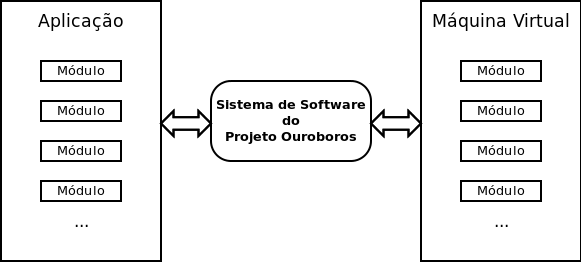
\includegraphics[width=.8\textwidth]{overview-simple.png}
      \caption{Esquematização bem simplificada do funcionamento sistema.}
      \label{fig:overview-simple}
    \end{figure}

    Dessa forma, uma primeira ilustração bem simplificada do funcionamento do
    nosso sistema é a representada na Figura \ref{fig:overview-simple}. O
    sistema Ouroboros será responsável por fornecer acesso aos módulos entre a
    aplicação e as máquinas virtuais. Dessa forma, estabelecemos duas
    grandes funcionalidades no sistema: providenciar à aplicação a possibilidade
    de manipular os módulos das máquinas virtuais, e deixar os módulos da
    aplicação à disposição dos \script{s} . Esses processos são conhecidos como
    \textbf{incorporação}\footnote{Do inglês, ``\textit{embedding}''.} e
    \textbf{exportação}, respectivamente.

    \definicao{
      \vspace{-1.5em}
      \begin{enumerate}
        \item \textbf{Incorporação} é quando a aplicação programada na linguagem
              nativa pode acessar e manipular os elementos dos módulos da
              máquina virtual.
        \item \textbf{Exportação} é quando módulos da aplicação na linguagem
              nativa são registrados na máquina virtual de modo que os módulos
              desta possam usar funcionalidades daquela.
      \end{enumerate}
    }

    Nesse ponto vale à pena destacar um aspecto que ficou de lado até agora.
    Como o subtítulo desse trabalho indica, o propósito do sistema é não só
    integrar as ditas linguagens, como fazê-lo de maneira \textit{automatizada}.
    Até porque as APIs das máquinas virtuais por sí sós possuem seus próprios
    mecanismos de fornecer incorporação e exportação, indicando que nosso
    projeto seria redundante, não fosse o fato que elas são trabalhosas e
    específicas demais de usar. A intenção é que o usuário do nosso sistema não
    tenha que se preocupar com os detalhes de cada máquina virtual quando
    estiver desenvolvendo a aplicação dele e seja capaz de escrever normalmente
    os \script{s} que trabalhem com ela - isso é, podendo acessar módulos
    externos através dos mecanismos usuais que a linguagem virtual fornece.

    Logo, nosso sistema consistirá majoritariamente de uma biblioteca \CXX{}
    que disponibiliza incorporação e exportação automatiza de e para \script{s}.
    Faremos isso aproveitando as possibilidades de abstração da linguagem
    escolhida para encapsular os comportamentos desejados. As duas próximas
    sessões explicarão como projetamos as partes dessa biblioteca que atenderão
    cada um desses requisitos.

  \section{API unificada para incorporação de \script{s}}
  \label{cap:estrutura:opa}

    Como vimos na sessão \ref{cap:conceitos:apis}, as máquinas virtuais com que
    estamos trabalhando possuem uma API própria através da qual podemos
    manipular seu conteúdo. Para evitar que o usuário acesse elas diretamente
    (e tenha que lidar com os mecanismos dela ele mesmo), podemos encapsulá-las
    por trás de uma camada que constitua uma nova API. Ela unificará o acesso às
    funcionalidades de todas as máquinas virtuais compatíveis. Mais
    especificamente, ela fornecerá os seguintes serviços:

    \begin{enumerate}
      \item Carregar um módulo a partir de um \script{};
      \item Executar rotinas implementadas na linguagem virtual;
      \item Acessar objetos definidos na linguagem virtual;
      \item Converter valores entre tipos da linguagem nativa e tipos da
            linguagem virtual;
    \end{enumerate}

    Idealmente, quando o usuário requisitar um desses serviços, ele não precisa
    saber qual máquina virtual realmente vai atendê-lo. Em termos práticos, isso
    significa que quando ele evocar a rotina que representa o serviço desejado,
    queremos que na verdade a rotina executada seja aquela que corresponda à
    máquina virtual apropriada ``sem que ele perceba'', como na figura
    \ref{fig:api-unificada}. Ou seja, precisamos de funções com nomes e
    assinaturas\footnotemark{} fixos simbolizando a operação almejada, porém
    sobrecarregadas com implementações circunstancialmente diferentes. Um jeito
    de obter esse efeito em \CXX{} é através da herança de classes, que é o
    método que adotaremos. Basicamente, sempre que formos implementar uma
    funcionalidade que dependa do funcionamento das máquians virtuais,
    definiremos uma classe abstrata com as assinaturas desejadas e herdaremos
    ela em classes específicas para cada linguagem de \script{}, que
    implementarão o que de fato acontece quanda as funções da classe original
    são chamadas. Quando objetos dessas classes forem instanciados, os
    mecanismos de \CXX{} garantirão que a implementação usada corresponderá à
    classe verdadeira deles (relativa a alguma máquina virtual), por mais que a
    aplicação do usuário só conheça a classe abstrata mãe.

    \footnotetext{
      A \emph{assinatura} de uma rotina ou função especifica que tipos de
      parâmetros ela recebe e que tipos de valores ela devolve a quem a
      evocou.
    }

    \begin{figure}[ht]
      \centering
      \caption{}
      \begin{subfigure}{.8\textwidth}
        \begin{center}
          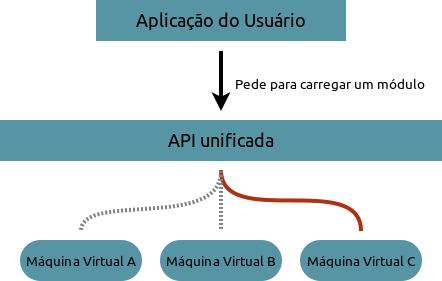
\includegraphics[width=.5\textwidth]{api-unificada.png}
          \vspace{1em}

          \textit{
            Nesse exemplo, a aplicação do usuário pede para carregar um certo
            módulo \script{}. A API unificada deve discernir qual máquina virtual
            é a apropriada para tal (no caso, a máquina C) e delegar a tarefa, sem
            que o usuário precise saber.
          }
        \end{center}
      \end{subfigure}
      \label{fig:api-unificada}
    \end{figure}

    Vamos, então, usar os serviços listados acima para escolher a combinação de
    classes que a API unificada oferecerá. Uma maneira de fornecer acesso a
    objetos virtuais, como especifica o item 3, é encapsular seu comportamento
    em uma classe própria. Dessa forma, quando instâncias dessa classe fossem
    manipuladas pela aplicação do usuário, elas internamente executariam as
    operações necessárias na máquina virtual para que o efeito desejado
    refletisse nela. E com isso ganhamos o item 4 de graça, pois basta colocar
    nessa classe métodos que convertam o valor interno do objeto virtual para
    \CXX{} e vice-versa. Por exemplo, o usuário poderia usar uma instância dessa
    classe para referir-se a uma cadeia de caracteres definida em um \script{}
    para convertê-la para o tipo \lang{string} em \CXX{}. O item 2 também
    é facilmente satisfeito pois, levando em consideração que nas linguagens de
    \script{} com que estamos trabalhando funções são tipos de primeira
    classe\footnotemark{}, um objeto virtual também seria capaz de conter uma
    delas de forma que ao ser evocado desencadearia a rotina correspondente
    dentro da máquina virtual. A figura \ref{fig:api-vobjs} exemplifica essas
    ideias.

    \footnotetext{
      Quando funções são tipos de \emph{primeira classe}, elas podem ser
      tratadas como se fossem um valor, o que permite que elas possam ser
      armazenadas em variáveis, passadas como argumento para outras funções
      e até mesmo devolvidas por outras funções também.
    }

    Fica faltando apenas o item 1, com o qual podemos seguir o mesmo raciocínio
    que usamos com funções: podemos tratar módulos como objetos virtuais. Assim,
    quando o usuário pede para carregar um \script{}, ele recebe uma instância
    de objeto virtual que abstrai o módulo em si. Isso exige que a classe
    tenha operações de acesso a membros dos objetos, para a aplicação poder
    alcançar os objetos virtuais que estão ``dentro'' do módulo. Para completar,
    a técnica de sobrecarga via herança nos permite criar, para cada máquina
    virtual, implementações diferentes dessa classe que representa objetos
    virtuais e mesmo assim exigir que o usuário use apenas uma classe base com
    as assinaturas de todas essas operações que vimos. 

    \begin{figure}[ht]
      \centering
      \caption{}
      \begin{subfigure}{.8\textwidth}
        \begin{center}
          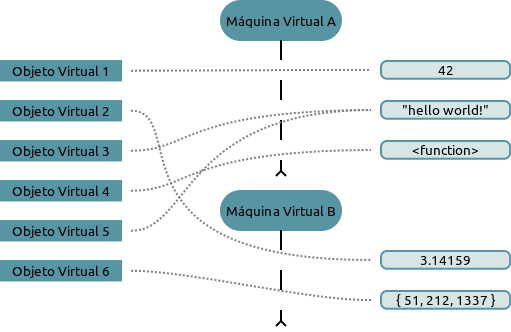
\includegraphics[width=.7\textwidth]{api-vobjs.png}
          \vspace{1em}

          \textit{
            Cada instância da classe que representará objetos virtuais encapsula
            um valor dentro de alguma máquina virtual. Note que mais de uma
            instância pode interagir com um mesmo valor.
          }
        \end{center}
      \end{subfigure}
      \label{fig:api-vobjs}
    \end{figure}

    Por uma questão de projeto de código, são necessárias ainda mais duas
    classes. Afinal, quando o usuário quiser carregar um módulo para obter seu
    respectivo objeto virtual, que parte da nossa API ele deverá usar? A classe
    dos objetos virtuais não pode ser instanciada sozinha (até porque ela é
    abstrata). Normalmente, quem tem as informações necessárias para tanto são
    as própsicas máquinas virtuais. Então, uma solução seria definir uma classe
    para as máquinas virtuais também, novamente usando herança para abstrair o
    funcionamento delas ao mesmo tempo deixando assinaturas relevantes ficam
    expostas. A terceira classe seria justamente para gerenciar as instâncias de
    máquinas virtuais. As relações entre essas três classes e o usuário estão
    representadas na figura \ref{fig:api-classes}.

    Chamamos a parte do nosso sistema que corresponde a essa API unificada de
    \emph{\textbf{Ouroboros Project API}} ou simplesmente \textbf{OPA}.

    \begin{figure}[ht]
      \centering
      \caption{}
      \begin{subfigure}{.8\textwidth}
        \begin{center}
          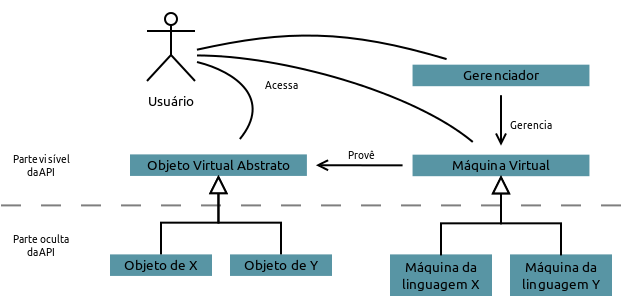
\includegraphics[width=\textwidth]{api-classes.png}
          \vspace{1em}

          \textit{
            Isso não chega a ser uma diagrama UML, apenas uma representação
            simbólica das classes. A especificação mais detalhada delas será
            exposta no capítulo \ref{cap:atividades}. Mas emprestamos a notação
            de herança.
          }
        \end{center}
      \end{subfigure}
      \label{fig:api-classes}
    \end{figure}
  
  \section{Gerador de \textit{wrappers} para exportação de interfaces nativas}
  \label{cap:estrutura:opwig}

    Para entender melhor como fazer a exportação, precisamos saber o que
    exportar. No caso, como as aplicações dos usuários estarão escritas em \C{}
    ou \CXX{}, os elementos que gostaríamos de exportar serão:

    \begin{enumerate}
      \item Variáveis globais.
      \item Funções globais.
      \item Tipos novos definidos na aplicação (usando \lang{typedef}, classes
            ou equivalentes)
      \item Outras informações, como \textit{namespaces}.
    \end{enumerate}

    No terceiro item, o ideal é que todas as operações inerentes ao tipo
    também sejam exportadas. Isso englobaria tanto operações aritméticas básicas
    quanto os métodos de classes, por exemplo. O usuário deverá ser capaz de
    criar objetos desses tipos em seus \script{s} e usá-los da maneira mais fiel
    possível ao modo como eles seriam usados no código nativo da aplicação.

    O que explicamos nas sessões \ref{cap:conceitos:apis:lua} e
    \ref{cap:conceitos:apis:python} nos fornece algumas ferramentas úteis,
    apesar de trabalhosas, para exportar esses elementos que listamos.
    Basicamente, podemos usar os mecanismos de registro de módulos nas máquinas
    virtuais para expor os módulos reais da aplicação\footnotemark{}. Aproveitando
    o exemplo que demos na seção \ref{cap:estrutura:geral}, poderia haver um
    módulo na aplicação (no caso, um jogo) que cuidasse do posicionamento de
    avatares, e nós gostaríamos que \script{s} incorporados pudessem acessar
    suas funcionalidades. Todas as variáveis, funções e tipos relacionados
    teriam que ser colocados no módulo virtual através das funções de
    inicialização, que precisam ser feitas usando o protocolo esperado pelas
    APIs.

    \footnotetext{
      Para não confundir a qual tipo de módulo estaremos nos referindo,
      chamaremos os módulos que registramos nas máquinas virtuais de
      \emph{módulos virtuais}, enquanto que os da aplicação serão simplesmente
      \emph{módulos}.
    }

    Isso compõe um método de exportação que funciona, mas traz dificuldades. A
    maior delas é que \C{} e \CXX{} não oferecem um meio de definir funções
    novas em tempo de execução, impedindo nossa biblioteca de registrar módulos
    virtuais durante suas rotinas, pois as funções de inicialização já precisam
    estar criadas quando a aplicação do usuário for ser compilada. A outra
    grande dificuldade é que é igualmente impossível de analisar o código da
    aplicação durante a execução dela mesma dadas as linguagens compiladas que
    adotamos. Normalmente, se um desenvolvedor quisesse exportar seu código
    nativo para uma linguagem de \script{}, ele simplesmente escreveria as
    funções de inicialização e manualmente colocaria cada elemento do código
    dele nos módulos exportados. Mas o que estamos tentando projetar aqui visa
    justamente \emph{automatizar} a integração aplicação-\script{s}, então
    simplesmente pedir para o usuário fazer esse trabalho sujo para nós está
    fora de questão. Assim sendo, não temos como saber quais variáveis, funções
    e tipos pertencem a um módulo e, mesmo que soubéssemos, não temos como
    fornecer as funções de inicialização necessárias quando a aplicação do
    usuário for executada e esse serviço for requerido da nossa biblioteca.
    
    Um jeito de contornar esses problemas é \emph{não} tentar fazer a exportação
    durante a execução da aplicação, mas sim antes de ela ser compilada, de
    maneira que tenhamos acesso ao código fonte dela. A partir dele somos
    capazes de reconhecer as declarações que queremos importar, e podemos
    escrever o código adicional das funções de inicialização a tempo
    de elas serem compiladas junto com o resto da aplicação. Isso seria feito
    por um outro programa - que obviamente precisa estar compilado antes da
    aplicação, uma vez que ele \emph{interfere} com o código dela - que chamamos
    de \emph{gerador de código}. Na prática, as únicas partes do código da
    aplicação que ele precisa analisar são os cabeçalhos, que é onde estarão as
    declarações. Uma visão geral desse procedimento está ilustrada na figura
    \ref{fig:gerador-funcionamento}.

    No entanto, ainda sobram algumas outras complicações porque, em geral,
    elementos nativos não podem ser exportados diretamente. Isso fica bastante
    claro quando olhamos para o modo como funções nativas são passadas para as
    máquinas virtuais: elas precisam ter uma assinatura específica, que ainda
    por cima varia de máquina para máquina. E fica ainda mais complicado quando
    pensamos em classes, pois em \lang{Lua}, por exemplo, não há orientação a
    objetos implementada por padrão - embora seja possível construir mecanismos
    na linguagem que funcionem como classes, que é o que precisamos fazer.

    \begin{figure}[ht]
      \centering
      \caption{}
      \begin{subfigure}{.8\textwidth}
        \begin{center}
          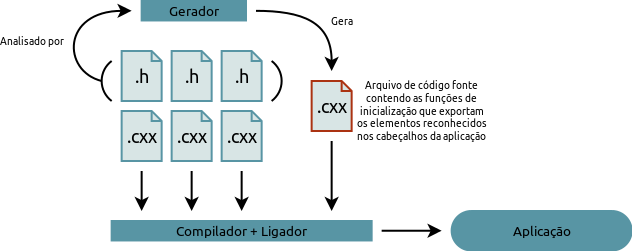
\includegraphics[width=\textwidth]{gerador-funcionamento.png}
          \vspace{1em}

          \textit{
            Representação de como o gerador conribui na exportação.
            Em \CXX{}, arquivos de cabeçalho usam a extensão \lang{.h} enquanto
            que arquivos de implementação usam \lang{.cxx}, embora haja outras
            conveções.
          }
        \end{center}
      \end{subfigure}
      \label{fig:gerador-funcionamento}
    \end{figure}

    Então, para cada tipo de elemento nativo que estamos interessados
    (variáveis, funções, tipos, etc), precisamos de uma maneira de adaptá-los
    para o formato que as máquinas virtuais esperam. Isso é possível através do
    uso de \textit{wrappers} (do inglês, ``embrulhos''), que nesse contexto são
    porções de código que encapsulam as atividades nativas da aplicação para
    expô-los adequadamente aos protocolos que as APIs das máquinas virtuais
    exigem para exportação. Assim, o que realmente estaremos inserindo nos
    módulos virtuais serão esses \textit{wrappers}, e não os elementos
    originais. Entraremos em mais detalhes sobre como fazer esses wrappers no
    capítulo \ref{cap:atividades}. Por enquanto, o importante é entender que
    essa parte do nosso sistema envolverá um gerador de código que produzirá
    os \textit{wrappers} que ele julgar necessário dado o código fonte da
    aplicação do usuário, e os inserirá em módulos virtuais de maneira a
    efetivamente exportar as funcionalidades nativas para as máquinas virtuais.

    Isso tudo significa que no final das contas nosso sistema não será apenas
    uma biblioteca, pois ele também terá executáveis fazendo o papel de
    geradores, um para cada linguagem de \script{}. O que fizemos para evitar
    espalhar muito nosso código é que esses programas auxiliares simplesmente
    evocam algumas rotinas da nossa biblioteca que de fato farão a análise e
    a geração de código. Chamamos essa parte do nosso sistema de \emph{Ouroboros
    Project Wrapper and Interface Generator} (OPWIG).

